

\section{Background}

\begin{frame}{Uniqueness of Movie Dubbing Task}
 \textbf{Movie dubbing}: Convert scripts to speeches, aligning with clip in timing and emotion, while preserving reference audio's timbre.\cite{zhang2024speaker}
    \begin{columns}[c]
        \column{0.6\textwidth}
        \begin{itemize}
            \item \textbf{Traditional VC/TTS}: Rely on the input text for modeling.
            \item \textbf{Movie dubbing}: Align with clip in emotion, rate, lip movements; preserve vocal timbre.
            \item \textbf{Transformed to one-to-one mapping.}
        \end{itemize}
        \column{0.4\textwidth}
        \begin{figure}
            \centering
            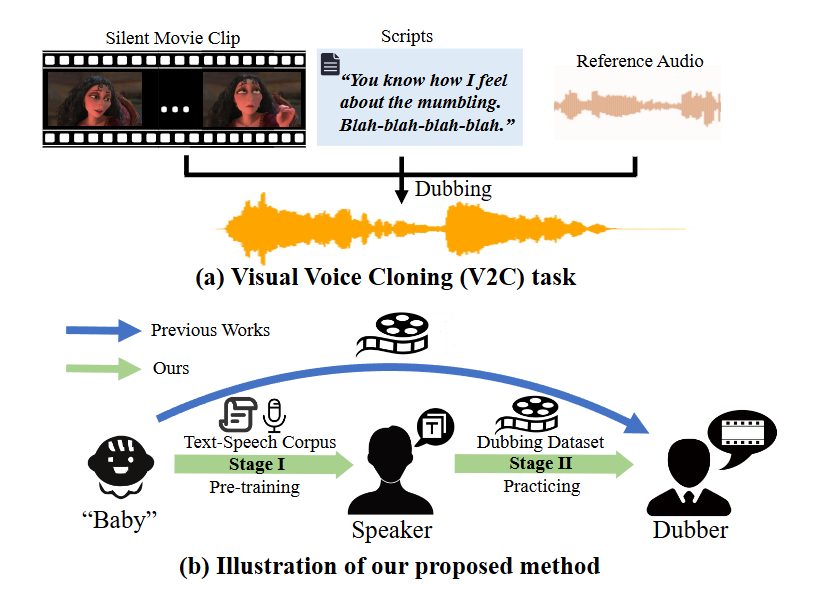
\includegraphics[width=\linewidth]{figs/difference.png}
            \caption{Movie dubbing vs. traditional VC/TTS}
            \label{fig:v2c_task}
        \end{figure}
    \end{columns}
\end{frame}


% \begin{frame}{Objectives of Movie Dubbing Task}
% \begin{columns}
%     \begin{column}{0.6\textwidth}
%         \begin{itemize}
%             \item Objectives of the movie dubbing task:
%             \begin{itemize}
%                 \item Preserve vocal timbre: Ensure a high match between the timbre of the dubbed speech and the reference audio.
%                 \item Synchronize emotion and speech rate: Align the emotional expression and speech rate of the dubbing with the performance of the characters in the movie clip.
%                 \item Align lip movements with speech: Match the duration of each phoneme in the dubbing with the lip movements of the characters.
%             \end{itemize}
%             \item The model needs to adapt to variations in emotion and speech rate while maintaining accurate pronunciation.
%         \end{itemize}
%     \end{column}
%     \begin{column}{0.4\textwidth}
%         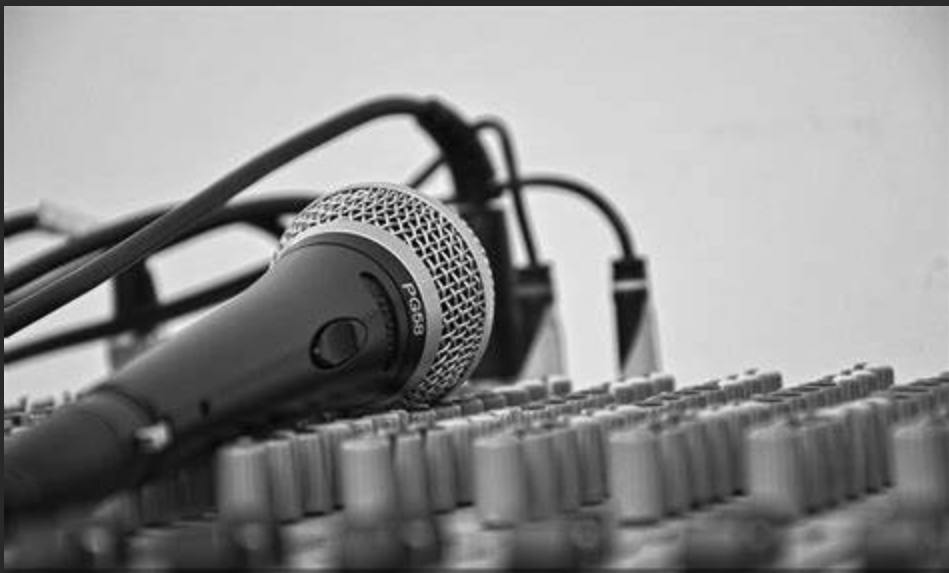
\includegraphics[width=\textwidth]{figs/配音.png} % Keep the original image path
%     \end{column}
% \end{columns}
% \end{frame}


\begin{frame}{Objectives of Movie Dubbing Task}
\textbf{The model needs to adapt to changes in emotion and speech speed to keep pronunciation accurate.}
\begin{columns}
    \begin{column}{0.6\textwidth}
        \begin{itemize}
                \item \textbf{Timbre}: Match dubbed speech to reference audio.
                \item \textbf{Emotion \& Rate}: Align with movie characters' performance.
                \item \textbf{Lip Sync}: Match phoneme duration to lip movements.
        \end{itemize}
    \end{column}
    \begin{column}{0.4\textwidth}
        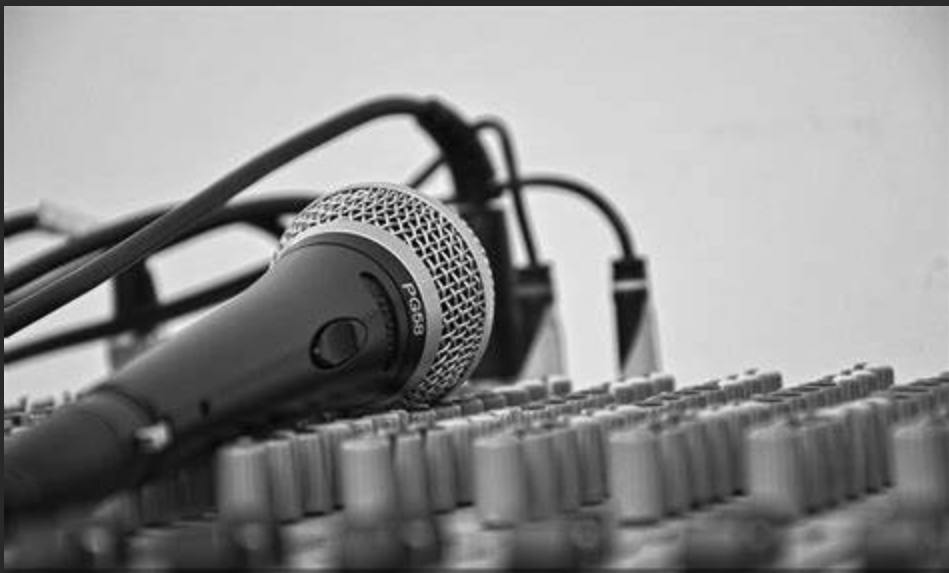
\includegraphics[width=\textwidth]{figs/配音.png}
    \end{column}
\end{columns}
\end{frame}



% \begin{frame}{Related Work}
% The Visual Voice Cloning (V2C) task \cite{chen2022v2c} requires the generated dubbing to align with the video content in terms of lip movements, emotions, and duration, which makes traditional speech synthesis methods inapplicable. To enhance the naturalness and consistency of dubbing, the authors draw on pre-training strategies and multi-modal alignment techniques.
% \begin{itemize}
% \item \textbf{Speech Synthesis:} Existing methods (e.g., the FastSpeech series) \cite{ren2020fastspeech} have made significant progress in speech synthesis, but they lack modeling of prosody and duration consistency with video content and thus cannot be directly applied to the V2C task.
% \item \textbf{Visual Voice Cloning:} The V2C task demands that the generated dubbing align with the video content in lip movements, emotions, and duration, significantly increasing the complexity of the task.
% \item \textbf{Pre-training in Text-to-Speech:} Pre-training strategies such as MP-BERT \cite{zhang2022mixed} and PLBERT \cite{li2023phoneme} enhance the naturalness of speech generation through phoneme-level modeling. These strategies are introduced into the V2C task in this paper to improve the quality of dubbing.
% \end{itemize}
% \end{frame}


\begin{frame}{Related Work}
The Visual Voice Cloning (V2C) task \cite{chen2022v2c} requires the generated dubbing to align with the video content in terms of lip movements, emotions, and duration, which makes traditional speech synthesis methods inapplicable. 
\begin{itemize}
    \item \textbf{Speech Synthesis:} FastSpeech\cite{ren2020fastspeech} series  excel in speech synthesis but lack video content alignment, making them unsuitable for V2C.
    \item \textbf{Visual Voice Cloning (V2C) :} Requires lip sync, emotion, and duration alignment with video, increasing task complexity.\cite{chen2022v2c}
    \item \textbf{Pre-training in TTS:} Strategies like MP-BERT \cite{zhang2022mixed} and PLBERT \cite{li2023phoneme} enhance speech naturalness via phoneme-level modeling, adopted in V2C to improve dubbing quality.
\end{itemize}
\end{frame}